\documentclass[11pt,letterpaper]{article}
\usepackage[lmargin=1in,rmargin=1in,tmargin=1in,bmargin=1in]{geometry}
\usepackage{../style/homework}
\usepackage{../style/commands}
\setbool{quotetype}{true} % True: Side; False: Under
\setbool{hideans}{false} % Student: True; Instructor: False

% -------------------
% Content
% -------------------
\begin{document}

\homework{1: Due 02/08}{Windows are the eyes to the house.}{Andy Dwyer, Parks \& Recreation}

% Problem 1
\problem{10} Give the definition of a real number. Also, give at least five original examples of a real number. \pspace

{\itshape A real number is `any' number which is expressible as a decimal, e.g.
	\[
	\begin{aligned}
	0&= 0.0 \\[0.3cm]
	1&= 1.0 \\[0.3cm]
	-5&= -5.0 \\[0.3cm]
	\dfrac{1}{2}&= 0.5 \\[0.3cm]
	-\dfrac{1}{10}&= -0.1 \\[0.3cm]
	0.119589&04771 \\[0.3cm]
	\sqrt{2}= 1.4142135&62373095\ldots \\[0.3cm]
	\pi= 3.14159265&3589793\ldots \\[0.3cm]
	e= 2.71828182&8495045\ldots \\[0.3cm]
	\gamma= 0.577215&664901532\ldots
	\end{aligned}
	\]
}



\newpage



% Problem 2
\problem{10} Give the definition of a rational number. Also, give at least five original examples of a rational number. \pspace

{\itshape A rational number is a real number of the form $\frac{a}{b}$, where $a$ and $b$ are integers and $b \neq 0$, e.g.
	\[
	\begin{aligned}
	0&= \dfrac{0}{1} \\[0.3cm]
	2&= \dfrac{2}{1} \\[0.3cm]
	-5&= -\dfrac{5}{1} \\[0.3cm]
	\phantom{=}& \dfrac{1}{2} \\[0.3cm]
	-\phantom{=}&\dfrac{5}{7} \\[0.3cm]
	\phantom{.}&\dfrac{20}{100} 
	\end{aligned}
	\]
}



\newpage



% Problem 3
\problem{10} Find the prime factorizations of the following integers:
	\begin{enumerate}[(a)]
	\item $54$
	\item $97$
	\item $168$
	\item $184$
	\end{enumerate} \pspace

\sol
\begin{enumerate}[(a)]
\item $54= 2 \cdot 3^3$
	\[
	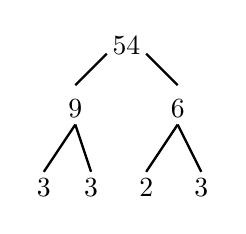
\begin{tikzpicture}
	\node at (-0.15,0) {$54$};
	\draw[line width=0.03cm] (-0.4,-0.1) -- (-0.8,-0.5);
	\node at (-0.8,-0.8) {$9$};
	\draw[line width=0.03cm]  (0.1,-0.1) -- (0.5,-0.5);
	\node at (0.5,-0.8) {$6$};
		
	\draw[line width=0.03cm] (-0.8,-1) -- (-1.2,-1.6);
	\node at (-1.2,-1.8) {$3$};
	\draw[line width=0.03cm] (-0.8,-1) -- (-0.6,-1.6);
	\node at (-0.6,-1.8) {$3$};
	
	\draw[line width=0.03cm] (0.5,-1) -- (0.1,-1.6);
	\node at (0.1,-1.8) {$2$};
	\draw[line width=0.03cm] (0.5,-1) -- (0.8,-1.6);
	\node at (0.8,-1.8) {$3$};
	\end{tikzpicture}
	\] \pspace
	
\item $97= 97$ (Already prime) \pspace

\item $168= 2^3 \cdot 3 \cdot 7$
	\[
	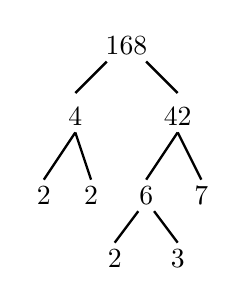
\begin{tikzpicture}
	\node at (-0.15,0.1) {$168$};
	\draw[line width=0.03cm] (-0.4,-0.1) -- (-0.8,-0.5);
	\node at (-0.8,-0.8) {$4$};
	\draw[line width=0.03cm]  (0.1,-0.1) -- (0.5,-0.5);
	\node at (0.5,-0.8) {$42$};
		
	\draw[line width=0.03cm] (-0.8,-1) -- (-1.2,-1.6);
	\node at (-1.2,-1.8) {$2$};
	\draw[line width=0.03cm] (-0.8,-1) -- (-0.6,-1.6);
	\node at (-0.6,-1.8) {$2$};
	
	\draw[line width=0.03cm] (0.5,-1) -- (0.1,-1.6);
	\node at (0.1,-1.8) {$6$};
	\draw[line width=0.03cm] (0.5,-1) -- (0.8,-1.6);
	\node at (0.8,-1.8) {$7$};
	
	\draw[line width=0.03cm] (0,-2.0) -- (-0.3,-2.4);
	\node at (-0.3,-2.6) {$2$};
	\draw[line width=0.03cm] (0.2,-2.0) -- (0.5,-2.4);
	\node at (0.5,-2.6) {$3$};
	\end{tikzpicture}
	\] \pspace

\item $184= 2^3 \cdot 23$
	\[
	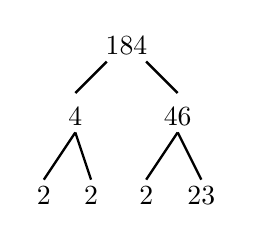
\begin{tikzpicture}
	\node at (-0.15,0.1) {$184$};
	\draw[line width=0.03cm] (-0.4,-0.1) -- (-0.8,-0.5);
	\node at (-0.8,-0.8) {$4$};
	\draw[line width=0.03cm]  (0.1,-0.1) -- (0.5,-0.5);
	\node at (0.5,-0.8) {$46$};
		
	\draw[line width=0.03cm] (-0.8,-1) -- (-1.2,-1.6);
	\node at (-1.2,-1.8) {$2$};
	\draw[line width=0.03cm] (-0.8,-1) -- (-0.6,-1.6);
	\node at (-0.6,-1.8) {$2$};
	
	\draw[line width=0.03cm] (0.5,-1) -- (0.1,-1.6);
	\node at (0.1,-1.8) {$2$};
	\draw[line width=0.03cm] (0.5,-1) -- (0.8,-1.6);
	\node at (0.8,-1.8) {$23$};
	\end{tikzpicture}
	\] 
\end{enumerate}



\newpage



% Problem 4
\problem{10} Without using a calculator, answer the following:
	\begin{enumerate}[(a)]
	\item Does 2 divide 2346? Explain.
	\item Does 3 divide 596012? Explain.
	\item Does 4 divide 990140? Explain.
	\item Does 5 divide 1431? Explain.
	\item Does 9 divide 70155? Explain. 
	\end{enumerate} \pspace

\sol
\begin{enumerate}[(a)]
\item We know that an integer is divisible by 2 if and only if the integer is even. Because 2346 is even, we know that it is divisible by 3. In fact, $2346= 1173(2)$. 

\item We know that an integer is divisible by 3 if and only if the sum of the digits is divisible by 3. Because $5 + 9 + 6 + 0 + 1 + 2= 23$, which is not divisible by 3, the integer 569012 is not divisible by 3. In fact, $596012/3 \approx 198670.667$. 
 
\item We know that an integer is divisible by 4 if and only if the last two digits of the integer is divisible by 4. Because 40  is divisibly by 4, we know that 990140 is divisible by 4. In fact, $990140= 247535(4)$. 

\item We know that an integer is divisible by 5 if and only if the integer ends in a 0 or a 5. Because 1431 ends in a 1, we know that 1431 is not divisible by 5. In fact, $1431/5= 286.2$.

\item We know that an integer is divisible by 9 if and only if the sum of the digits is divisible by 9. Because $7 + 0 + 1 + 5 + 5= 18$, which is divisible by 9, the integer 70155 is divisible by 9. In fact, $70155= 7795(9)$. 
\end{enumerate}



\newpage



% Problem 5
\problem{10} Using the `square root method,' show that 157 is prime. \pspace

\sol We know that if a positive integer $N$ is composite that it has a factor at most $\sqrt{N}$. Observe that $\sqrt{157} \approx 12.53$. Therefore, if 157 is composite, i.e. not prime, then it must have a prime divisor between 2 and 12. We check to see if any of the prime numbers between 2 and 12, i.e. 2, 3, 5, 7, and 11, divide 157: \par
	\begin{table}[!ht]
	\centering
	\begin{tabular}{r|rrrrr}
	Prime & 2 & 3 & 5 & 7 & 11 \\ \hline
	Divisible & \xmark & \xmark & \xmark & \xmark & \xmark
	\end{tabular}
	\end{table} \par
But then 157 does not have a prime divisor $\leq 12$. Therefore, 157 cannot be composite, i.e. 157 is prime. 



\newpage



% Problem 6
\problem{10} By listing out all the divisors of the given numbers, compute the following:
	\begin{enumerate}[(a)]
	\item $\gcd(12, 15)$
	\item $\gcd(20, 22)$
	\item $\gcd(36, 60)$
	\item $\gcd(20, 100)$
	\end{enumerate} \pspace

\sol
\begin{enumerate}[(a)]
\item \phantom{.}\par
	\begin{table}[!ht]
	\centering
	\begin{tabular}{rl}
	12: & 1, 2, \textbf{3}, 4, 6, 12 \\
	15: & 1, \textbf{3}, 5, 15
	\end{tabular}
	\end{table} \par
Therefore, $\gcd(12, 15)= 3$. \pspace

\item \phantom{.}\par
	\begin{table}[!ht]
	\centering
	\begin{tabular}{rl}
	20: & 1, \textbf{2}, 4, 5, 10, 20 \\
	22: & 1, \textbf{2}, 11, 22
	\end{tabular}
	\end{table} \par
Therefore, $\gcd(20, 22)= 2$. \pspace

\item \phantom{.}\par
	\begin{table}[!ht]
	\centering
	\begin{tabular}{rl}
	36: & 1, 2, 3, 4, 6, 9, \textbf{12}, 18, 36 \\
	60: & 1, 2, 3, 4, 5, 6, 10, \textbf{12}, 15, 20, 30, 60 
	\end{tabular}
	\end{table} \par
 Therefore, $\gcd(36, 60)= 12$. \pspace
 
\item \phantom{.}\par
	\begin{table}[!ht]
	\centering
	\begin{tabular}{rl}
	20: & 1, 2, 4, 5, 10, \textbf{20} \\
	100: & 1, 2, 4, 5, 10, \textbf{20}, 25, 50, 100
	\end{tabular}
	\end{table} \par 
Therefore, $\gcd(20, 100)= 20$. 
\end{enumerate}



\newpage



% Problem 7
\problem{10} By listing out sufficiently many multiples of the given integers, compute the following:
	\begin{enumerate}[(a)]
	\item $\lcm(24, 36)$
	\item $\lcm(12, 15)$
	\item $\lcm(12, 18)$
	\item $\lcm(36, 48)$
	\end{enumerate} \pspace

\sol
\begin{enumerate}[(a)]
\item  \phantom{.}\par
	\begin{table}[!ht]
	\centering
	\begin{tabular}{rl}
	24: & 24, 48, \textbf{72}, 96, 120, 144, 168, 192 \ldots \\
	36: & 36, \textbf{72}, 108, 144, 180, 216, 252, 288, \ldots
	\end{tabular}
	\end{table} \par 
Therefore, $\lcm(24, 36)= 72$. \pspace

\item  \phantom{.}\par
	\begin{table}[!ht]
	\centering
	\begin{tabular}{rl}
	12: & 12, 24, 36, 48, \textbf{60}, 72, 84, 96, \ldots \\
	15: & 15, 30, 45, \textbf{60}, 75, 90, 105, 120, \ldots
	\end{tabular}
	\end{table} \par 
Therefore, $\lcm(12, 15)= 60$. \pspace
 
\item  \phantom{.}\par
	\begin{table}[!ht]
	\centering
	\begin{tabular}{rl}
	12: & 12, 24, \textbf{36}, 48, 60, 72, 84, 96, \ldots \\
	18: & 18, \textbf{36}, 54, 72, 90, 108, 126, 144, \ldots
	\end{tabular}
	\end{table} \par 
Therefore, $\lcm(12, 18)= 36$. \pspace
 
\item  \phantom{.}\par
	\begin{table}[!ht]
	\centering
	\begin{tabular}{rl}
	36: & 36, 72, 108, \textbf{144}, 180, 216, 252, 288, \ldots \\
	48: & 48, 96, \textbf{144}, 192, 240, 288, 336, 384, \ldots
	\end{tabular}
	\end{table} \par  
Therefore, $\lcm(36, 48)= 144$. \pspace
\end{enumerate}



\newpage



% Problem 8
\problem{10} By finding prime factorizations, compute the following:
	\begin{enumerate}[(a)]
	\item $\gcd(12, 15)$
	\item $\gcd(20, 22)$
	\item $\gcd(36, 60)$
	\item $\gcd(20, 100)$
	\end{enumerate} \pspace

\sol
\begin{enumerate}[(a)]
\item 
	\[
	\gcd(12, 15)= \gcd(2^2 \cdot 3, 3 \cdot 5)= 3^1= 3
	\] \pspace

\item 
	\[
	\gcd(20, 22)= \gcd(2^2 \cdot 5, 2 \cdot 11)= 2^1= 2
	\] \pspace

\item 
	\[
	\gcd(36, 60)= \gcd(2^2 \cdot 3^2, 2^2 \cdot 3 \cdot 5)= 2^2 \cdot 3= 12
	\] \pspace

\item 
	\[
	\gcd(20, 100)= \gcd(2^2 \cdot 5, 2^2 \cdot 5^2)= 2^2 \cdot 5= 20
	\]
\end{enumerate}



\newpage



% Problem 9
\problem{10} By finding prime factorizations, compute the following:
	\begin{enumerate}[(a)]
	\item $\lcm(24, 36)$
	\item $\lcm(12, 15)$
	\item $\lcm(12, 18)$
	\item $\lcm(36, 48)$
	\end{enumerate} \pspace

\sol
\begin{enumerate}[(a)]
\item 
	\[
	\lcm(24, 36)= \lcm(2^3 \cdot 3, 2^2 \cdot 3^2)= 2^3 \cdot 3^2= 72
	\] \pspace

\item 
	\[
	\lcm(12, 15)= \lcm(2^2 \cdot 3, 3 \cdot 5)= 2^2 \cdot 3 \cdot 5= 60 
	\] \pspace

\item 
	\[
	\lcm(12, 18)= \lcm(2^2 \cdot 3, 2 \cdot 3^2)= 2^2 \cdot 3^2= 36
	\] \pspace

\item 
	\[
	\lcm(36, 48)= \lcm(2^2 \cdot 3^2, 2^4 \cdot 3^1)= 2^4 \cdot 3^2= 144
	\]
\end{enumerate}



\newpage



% Problem 10
\problem{10} Compute the following:
	\begin{enumerate}[(a)]
	\item $\gcd(2^3 \cdot 3^1 \cdot 5^3 \cdot 11^5, 2^2 \cdot 3^3 \cdot 5 \cdot 7)$
	\item $\lcm(2^3 \cdot 3^1 \cdot 5^3 \cdot 11^5, 2^2 \cdot 3^3 \cdot 5 \cdot 7)$
	\item $\gcd(2^{10} \cdot 5^5 \cdot 13, 3^5 \cdot 5^1 \cdot 11^2)$
	\item $\lcm(2^{10} \cdot 5^5 \cdot 13, 3^5 \cdot 5^1 \cdot 11^2)$
	\end{enumerate} \pspace

\sol
\begin{enumerate}[(a)]
\item 
	\[
	\gcd(2^3 \cdot 3^1 \cdot 5^3 \cdot 11^5, 2^2 \cdot 3^3 \cdot 5 \cdot 7)= 2^2 \cdot 3 \cdot 5= 60
	\] \pspace

\item 
	\[
	\lcm(2^3 \cdot 3^1 \cdot 5^3 \cdot 11^5, 2^2 \cdot 3^3 \cdot 5 \cdot 7)= 2^3 \cdot 3^3 \cdot 5^3 \cdot 7 \cdot 11^5= 30\ 438\ 639\ 000
	\] \pspace

\item 
	\[
	\gcd(2^{10} \cdot 5^5 \cdot 13, 3^5 \cdot 5^1 \cdot 11^2)= 5
	\] \pspace

\item 
	\[
	\lcm(2^{10} \cdot 5^5 \cdot 13, 3^5 \cdot 5^1 \cdot 11^2)= 2^{10} \cdot 3^5 \cdot 5^5 \cdot 11^2 \cdot 13= 1\ 223\ 164\ 800\ 000
	\]
\end{enumerate}


\end{document}